\documentclass[11pt,letterpaper]{article}
\usepackage{cogsys}
\usepackage{cogsysapa}
\usepackage[utf8]{inputenc}
\usepackage[T1]{fontenc}
\usepackage{times}
\usepackage[pdftex]{graphicx} % use this when importing PDF files

 % First page headings for accepted submissions.
%\cogsysheading{3}{2015}{1-16}{4/2015}{5/2015}
 % First page headings for poster submissions.
%\cogsysposterheading{Third}{2015}{1-16}
 % First page headings for workshop submissions.
\cogsysworkshopheading{2015}


\ShortHeadings{Interactive Knowledge-Goal Reasoning}
              {B.\ Bengfort and M.T.\ Cox}

\begin{document}

\title{Interactive Knowledge-Goal Reasoning}

\author{Benjamin Bengfort}{bengfort@cs.umd.edu}
\address{Department of Computer Science, University of Maryland,
         College Park, MD 20742 USA}
\author{Michael T. Cox}{michael.cox@wright.edu}
\address{Wright State Research Institute, Wright State University,
         Dayton, OH 45435 USA}
\vskip 0.2in

% Title (1000 readers)
% Abstract (4 sentences, 100 readers)
% Introduction (1 page, 100 readers)
% The problem (1 page, 10 readers)
% My idea (2 pages, 10 readers)
% The details (5 pages, 3 readers)
% Related work (1-2 pages, 10 readers)
% Conclusions and further work (0.5 pages)

\begin{abstract}
Knowledge goals are used by reasoning entities to fill in information required for decision making and are an important part of computational understanding systems. Simple knowledge goals can be solved through traditional information retrieval techniques or database queries. In order to solve complex knowledge goals, however, a plan must be composed and executed in an investigative manner. During computational investigation, goals of both the system and the user can change, resulting in goal trajectories that may inform future goal solutions. In this paper, we propose an interactive reasoning system that leverages a case-based methodology to solve complex knowledge goals represented as natural language queries.
\end{abstract}

\section{Introduction}

A \textit{knowledge goal} represents the purposeful need to acquire information in order to fill in gaps of world knowledge for a reasoning entity or to extend the database of a computational understanding system \cite{ram_goal-based_1991}. For humans, knowledge goals are most easily represented as questions, and current research on dialog-driven question and answer systems focuses on the semantic parsing of a natural language question to a structured database query \cite{yahya_natural_2012} or lambda calculus representation \cite{berant_semantic_2013}. These parsing approaches are making headway in the solution of simple knowledge goals, where the primary task is a retrieval from some structured knowledge base; especially goals that ask who, what, when, or where. This approach, however, cannot solve complex knowledge goals including aggregations, opinions (recommendations), or explanations for why or how questions. As a result, even though information retrieval systems and search have made information easily accessible, there has been the growth of community-driven question sites such as Quora \cite{wang_wisdom_2013} to connect users to the more nuanced answers they are looking for.

We claim that humans solve complex knowledge goals through \textit{investigation}, dividing harder questions into simpler sub-knowledge goals with more easily obtained solutions. When solving knowledge goals, humans also take into account context and approach new problems by leveraging techniques that have worked in the past. A system that models how humans investigate questions will \textit{deconstruct} a complex goal, \textit{integrate} relevant knowledge, and \textit{reuse} methods of investigation. Investigation can be represented as a plan to solve the larger knowledge goal, and if the tasks or subgoals of knowledge acquisition plans are simple knowledge goals that can be solved via structured data retrieval, then a system can be said to solve complex knowledge goals through a planning process that involves the purposeful combination of simpler knowledge goals.

In this paper we present a vision for an interactive knowledge-goal reasoning system that uses a case-based reasoning methodology to deconstruct complex knowledge goals based on previous cases for similar questions. The system will provide users with goal-driven solutions to natural language queries by proposing plans of simpler knowledge goals, which can be satisfied by computationally tractable tasks like database queries or document retrieval. The system takes into account the context of the goal by leveraging semantic resources applied to the question and utilizes a wide array of data sources to perform retrieval tasks--from database queries, to search, to providing other user responses for complex questions. As subtasks are selected by the initiating user, the case-based reasoning system reinforces and indexes how the plan was solved in order to provide more relevant plans or responses in the future.

Because this type of system is interactive and adaptive it is subject to goal changes, where the original knowledge goal is changed or refined slightly while the user interactively follows a solution plan. The complete case for solving a complex knowledge goal therefore represents a \textit{goal trajectory}. Goal trajectories are important for refining future cases, ranking plan solutions, and having the system anticipate knowledge goals to propose better plans. Furthermore, the combination of goal trajectories can be seen as a creative process, leading to the extension of not only the casebase, but also to extend automatically the knowledge base of the system.

%% Should I add the components (concept, task, context) of the question to the introduction?

To explore interactive knowledge-goal reasoning, we will first discuss knowledge goals and goal trajectories in detail. This discussion will lead to a brief taxonomy of questions, which is vital to understanding the many types of cases in a natural language query system. In the second section, we will describe our proposed case-based methodology, including the case representation, acquisition, and management. Finally, we will present three case studies that demonstrate how an interactive knowledge-goal reasoning system might be employed.

\section{Knowledge Goals}

In information retrieval systems, the input is a query that usually takes the form of a Boolean combination of keywords and the expected output is a ranked list of documents that have a high relevance to the keyword combination. Similarly, in database management systems the input is a formal query that must conform to the logical structure of the information, and the output is a set of records or aggregations that also conform to the schema. While these systems are important in the management of large-scale, multi-modal information sets, they do not represent the way that humans formulate knowledge goals: questions. Although search and structured database queries may be viewed as stand-ins for knowledge goals, they only embed the execution context or \textit{task} of the knowledge goal, whereas natural language queries express more information related to the goal and can be both \textit{simple} and \textit{complex} where formal languages are not as flexible.

We can define \textit{simple} knowledge goals as questions that are directly tied to a retrieval task and whose solution may be found either through traditional information retrieval or through structured queries. Consider the question ``\textit{Who won the World Cup?}'' The goal of this question is to determine the \texttt{Country} entity that won the most recent World Cup and possibly also the \texttt{Result} in the form of the competing teams and final score. Search methodologies would find documents with a high relevance to the tokens in the text of the question, particularly ``World Cup''. A structured database query upon some knowledge base would require semantic parsing to determine the relationship between the \texttt{FIFA World Cup} topic, and a specific \texttt{Country} topic. Even with these challenges, the result of both search and database query would fulfill the knowledge goal.

\textit{Complex} knowledge goals, on the other hand, cannot be solved simply through a single retrieval task and are generally related to questions that require investigation, opinion, explanation, or knowledge generation. Consider the question ``\textit{Where should I go to dinner?}'' This question is not a simple retrieval task because although restaurant reviews and geographic proximity searches might narrow the search space to dozens of possible candidate restaurants, selecting a dining option involves a reasoning process that may lead to solutions that do not involve restaurants at all, like going on a picnic. Moreover, this routine question will have different responses when asked by the same user multiple times, depending on context like geographic location, the season, or changing user preferences. Other complex knowledge goals are used to generate information, for example ``\textit{Can a crocodile complete a steeplechase?}'', a fact that is probably not part of most knowledge bases. Unless someone has already investigated this question, the goal will have to be decomposed into lines of questioning related to the physical requirements of completing a steeplechase compared to the athletic ability of crocodiles.

% Do we need more here?

\subsection{Knowledge Goal Representation}

The representation of a knowledge goal can be described by its objective: the type of the expected response (concept specification) and how the information will be used (task specification) \cite{ram_theory_1991}. To create a plan to solve a knowledge goal, a computational system must be able to represent knowledge goals in a structured manner, and identify and parse the structure from a natural language query. We extend this representation to leverage the additional components available in an interactive knowledge-goal reasoning system. Knowledge goals are composed of three primary features: a set of \textit{concepts}, a \textit{task}, and a specific \textit{context}. Each feature contributes to the solution as follows:

\begin{enumerate}

\item \textbf{Concept}: The knowledge goal is relevant to a specific set of structured semantic concepts, both entities and predicates, which are either directly specified or implied. The concept of the question identifies the domain of the query plan as well as the expected response.

\item \textbf{Task}: The task indicates the purpose of the knowledge goal and is usually implied in a natural language query and related to the motivation of the questioner. For example, in the case of simple knowledge goals the task may be search or database query; for more complex knowledge goals the task may be explanation or knowledge generation. It is by task that different types of knowledge goals are categorized in the taxonomy below.

\item \textbf{Context}: Knowledge goals are not specified in isolation, but are directly related to the questioner and as such must be considered in relation to their context. Contextual information includes temporal, geographic, hysteretic, and preference information and is essential for plan refinement and to resolve ambiguity.
\end{enumerate}

In the question ``\textit{When is the next flight to Paris?}'' the \textit{concept} explicitly includes the topic \texttt{Air Travel} as well as a city, \texttt{Paris}. Implied concepts might include \texttt{Paris, France}, the most popular city named Paris, and \texttt{Charles de Gaulle Airport}. The \textit{task} can generally be defined as a simple database query or search, but more specifically the return of a specific \texttt{Flight} record. The \texttt{context} is critical as well, especially the geographic context (the next flight to Paris from the city where the user is currently located) and the temporal context (in order to determine when the next flight might be).

Many applications simplify one or more components of a knowledge goal in order to be effective. Domain-specific applications reduce ambiguity in concepts and context by allowing only specifically relevant knowledge goals. More commonly, applications simplify the task and are designed to return only a single type of result. However, the widespread availability of large, general knowledge bases combined with timely contextual information from mobile devices mean that complete, personalized question and answer systems are becoming computationally tractable and knowledge goal simplification can no longer be used as an approximation for goal reasoning systems.

\subsection{Solving Knowledge Goals}

% Mention interactivity? %

An important step in the development of dialog-driven question and answer systems was the creation of large-scale structured knowledge bases like Freebase \cite{bollacker_freebase:_2008} and Yago2 \cite{suchanek_yago:_2007}. These databases represent a wealth of information generated from collaboratively edited encyclopedic sites like Wikipedia and provide the means with which to make factual queries about the world. Semantic parsers can take advantage of hierarchical, relational ontologies which allow for a generalization in the domain or \textit{concept} component of a question. For simple knowledge goals, semantic parsers can transform natural language questions into structured queries like SPARQL or SQL \cite{yahya_natural_2012}, a lambda-calculus representation \cite{berant_semantic_2013}, or simply a template from which to directly search other answers \cite{unger_template-based_2012}.

However, these parsers will struggle with even slightly more complex natural language queries tasked with a database lookup in a knowledge base, such as ``\textit{Who was the King of England when Thomas Jefferson was President?}'' This knowledge goal is a factual retrieval that can be solved by chaining subqueries to first solve which years Thomas Jefferson was President of the United States, then use the result to determine the King of England during that time period. Similarly, knowledge goals that require aggregation, such as ``\textit{How many countries have won three consecutive gold medals in a single sport?}'', may be able to be transformed into a series of simpler sub queries which contribute information to a final result.

The decomposition method of solving fact-based retrieval questions can also be applied to complex knowledge goals whose task is not simply a query or search. When a complex knowledge goal is reduced to one or more simpler sub goals, the result is a hierarchical plan to solve the original knowledge goal. If the final leaf nodes of such a plan are simple knowledge goals which can be transformed into a query or a search, then a system can said to solve complex knowledge goals through the computationally tractable combination of simpler knowledge goals.

\begin{figure}
	\centering
	    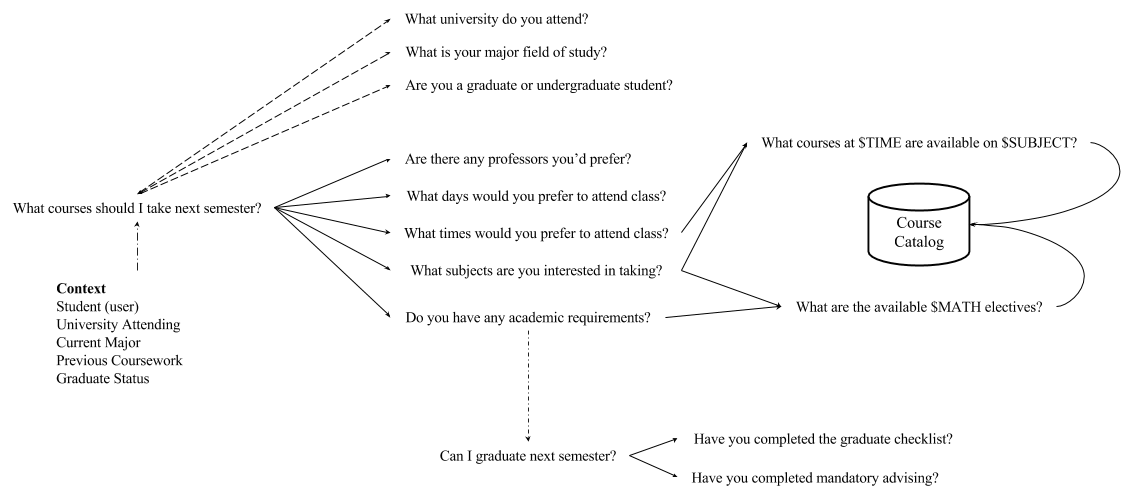
\includegraphics[width=\textwidth]{figures/simple_trajectory.png}
    \caption{\label{fig:simple_trajectory.png}Interactive knowledge goal reasoning on the complex goal, ``What courses should I take next semester?''. The system resolves context dependencies, then proposes a plan of simpler sub-goals that lead to database queries using information from prior goals (represented as \texttt{\small\$VAR)}. Depending on the interaction, a goal trajectory can modify the original goal to ``Can I graduate next semester?'', which continues the process.}
\end{figure}

Consider an example complex knowledge goal, ``\textit{What courses should I take next semester?}'', outlined in Figure \ref{fig:simple_trajectory.png}. This knowledge goal is routine, executed by the same user on a regular interval and common enough that a casebase of solutions is readily available. The task of this knowledge goal is to create a list of courses which are available next semester and which the student will presumably be able to register for. The concept of the question is the domain of courses that are available at a particular university during a particular semester. The context for a user determines preference in terms of the selected major or course level as well as geographical context (which specific university) and temporal context (which specific semester).

In order to solve this knowledge goal, a plan of simpler sub knowledge goals may be offered to the user. If contextual information is missing, the system might respond with ambiguity resolution goals of its own (e.g. ``\textit{Have you selected a major?}''). Otherwise simpler sub knowledge goals could include ``\textit{What days and times would you prefer?}'', ``\textit{Are there any academic subjects you're interested in?}'', or ``\textit{Do you have any academic requirements?}'' Responses to these sub-knowledge goals would lead to even simpler knowledge goals which can be eventually be queried against a course catalog, such as ``\textit{Which Economics courses are available on Monday and Wednesday?}''

\subsection{Goal Trajectories}

The solution to complex knowledge goals is an interactive reasoning approach where a complex knowledge goal is broken down into a hierarchical plan of simpler sub goals and tasks. In an interactive reasoning system, the user selects the next step of plans proposed by the reasoner, and continues to chain sub goals together to work towards a larger solution. During this process, the plan is adaptable and subject to change as the user proceeds in selecting and executing the simpler goals. Goals, like plans, are also subject to change and can be transformed \cite{cox_goal_1998}, therefore we propose that the original knowledge goal itself is also subject to change; and that as knowledge goals change during interactive reasoning, the path that led to the solution of new knowledge goals from the original can be represented by a \textit{goal trajectory}.

Goal trajectories can be influenced either through the direct interactive manipulation of goals \cite{cox_mixed-initiative_2007} or via other users in the system issuing similar queries that provide the basis for recommending new goals through collaborative filtering \cite{hayes_case-based_2001}. State changes in the system via monitoring of new information or relevant data that has been added to the knowledge base can also lead to new, interactive responses. In either case, goal changes can be seen as a planning problem where knowledge goals are not static, and an interactive reasoning system must be responsive to goal changes.

The concept of goal trajectories can then be used to explicitly define relationships between knowledge goals as cases for future solutions. In the example from Figure \ref{fig:simple_trajectory.png}, a goal trajectory is demonstrated by the proposed sub-knowledge goal, ``\textit{Do you have any academic requirements?}'', which leads the user to change the goal to ``\textit{Can I graduate next semester?}'' This goal trajectory can then be used in future cases to propose graduate related sub goals to those who may be close to finishing their degree.

\subsection{Knowledge Goal Taxonomy} \label{ssec:taxonomy}

In the next section, we will discuss the solution of knowledge goals by decomposing a complex knowledge goal into subsequently simpler knowledge goals. However, in order to determine an execution plan for knowledge goals, some idea of the types of knowledge goals that might be in a system as well as their relative complexity is required. Knowledge goals as described in \cite{ram_knowledge_1990,ram_goal-based_1991} are presented with a categorization based on the task that they arise from. Similarly, we will extend this taxonomy with our planning framework, given the components of a knowledge goal discussed in the last section.

\subsubsection{Simple Knowledge Goals}

The simplest knowledge goals should be computationally tractable, such that they can be solved with a minimal amount of user involvement. Simple knowledge goals have tasks that range from search to database queries to computational tasks like parsing, aggregation, or inference. In an \textit{interactive} system, both users and the system have simple knowledge goals. The system uses knowledge goals to resolve ambiguity through dialog boxes or through other types of feedback.

\begin{enumerate}

\item \textbf{Textual}: Questions related to both semantic or syntactic analysis of text, usually as a response to ambiguity. Tasks related to text questions include anaphora resolution or word sense disambiguation. Users may ask to define a word; the system may ask to clarify a concept.

\item \textbf{Contextual}: Questions designed to specify the result of a knowledge goal according to the user's context, such as queries related to preference, geography, or time. Similar to textual questions, these types of questions are "meta-questions" that are used to tailor the execution of a knowledge goal solution.

\item \textbf{Rhetorical}: Questions that should not return an answer. Questions that are used as placeholders or to express frustration are important to identify as simple knowledge goals because they identify terminal tasks in question plans.

\item \textbf{Retrieval}: Questions that expect a single fact returned from the database and may be transformed into a structured query. These types of questions may perform aggregations or filtering upon the knowledge base, but typically only return a single result or a small list of results.

\item \textbf{Search}: Questions that require a larger scope or domain and whose expected results are a list of relevant documents.

\end{enumerate}

The tasks related to these simple knowledge goals are all able to be computed on behalf of a user. Knowledge goals that fall into these categories are the simplest goals that may be involved in an interactive knowledge-goal reasoning system.

\subsubsection{Complex Knowledge Goals}

Complex knowledge goals must be reasoned upon rather than computed directly, and cannot be directly parsed into a executable representation. Instead, a plan must be developed in order to solve complex knowledge goals which leverages the context and concepts in the goal. The types of tasks for complex knowledge define the categorization of these goals as follows:

\begin{enumerate}

\item \textbf{Explanation}: Questions that require an explanation and return an explanatory data structure. Tasks include the detection and resolution of anomalies as well as the construction of an inferential or causal explanation.

\item \textbf{Relevance}: These questions are designed to expand the current knowledge framework by adding relevance links between questions and related entities, answers or other questions. Relevance can be used in later processing as a shortcut to retrieval from a casebase.

\item \textbf{Socratic}: Socratic questions return a question as an answer, or rather a plan that consists of knowledge goals that are designed to answer the larger question.

\item \textbf{Research}: These types of questions are designed to add information to a knowledge base, either by adding facts or creating knowledge from other knowledge sources. The system should identify research questions based on unsatisfactory queries and add them to the system for later investigation.

\item \textbf{Routine}: Questions that are routine are asked frequently or on a specific interval. However the required answer will differ based on the context or timing of the question and will most likely not return the same answer as a previous instance of the question.

\end{enumerate}

Tasks related to solving complex knowledge goals require some learning framework to mimic how humans solve similar goals. In an interactive reasoning system, the learning framework can include the use of similar cases or solutions to goals to propose a plan to solve the complex goal, or to connect related users as they investigate similar goals.

\section{Case-Based Reasoning for Knowledge Goals}

Our vision to solve complex knowledge goals is an \textit{interactive case-based reasoning system (CBR)} which reuses past experience \cite{kolodner_case-based_1993,lopez_de_mantaras_retrieval_2005}. Interactive CBR operates similarly to conversational case-based reasoning systems, which incrementally elicits a target problem through an interactive dialog with the user, attempting to minimize the number of questions before a solution is reached \cite{aha_advances_2005}. In order to provide an adaptable, investigative system, the methodology we are exploring guides the user through goal trajectories, removing the requirement to minimize session length in order to facilitate an ongoing discovery process. Additionally, the system itself is a learning agent with the goal of predicting future knowledge goals, and acquiring the information in advance.

\begin{figure}
	\centering
	    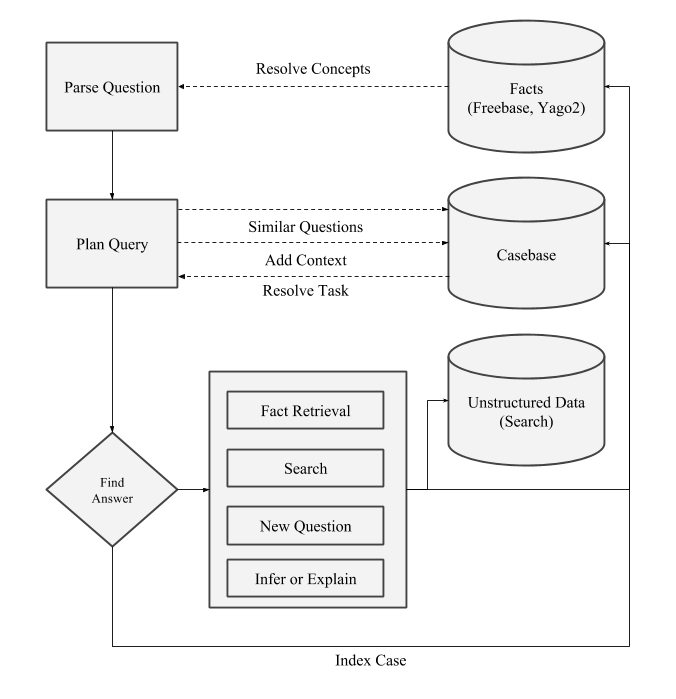
\includegraphics[width=\textwidth]{figures/architecture.png}
    \caption{\label{fig:architecture.png}An architecture for interactive knowledge-goal reasoning. The goal reasoning system decomposes complex knowledge goals expressed as natural language queries into plans of simpler goals.}
\end{figure}

An interactive knowledge-goal reasoning system would require the ability to correctly identify \textit{concepts} through some semantic parsing task. Knowledge goal \textit{concepts} would be used to identify similar knowledge goals in the casebase for retrieval. The system would also require the ability to classify the \textit{task} of the question in order to determine the execution context and to reuse previous cases. Finally the system would utilize the \textit{context} of the questioner to adapt or revise cases for the specific scenario. Knowledge goals and their trajectories would be retained in the casebase along with their relationships such that the system learns over time and can anticipate future knowledge goals, for example by detecting common goal trajectories and proposing shorter paths to those anticipated goals. The required components and architecture of such an interactive knowledge goal system are described in Figure \ref{fig:architecture.png}.

The input to the system is a natural language question, which is parsed to extract explicit topics defining the \textit{concept} of the question. Concepts involved in the question are directly tied to a structured knowledge base and ontology, providing the ability to query implicit concepts such as relationships to other topics or entities. Once the concepts have been resolved, the system leverages a casebase to find similar questions. Those similar questions will be adapted with the current context of the user, for example if the user asks ``\textit{When is the next home game?}'' the system can adapt previous questions regarding sporting events with seasonal context (football vs. baseball), or the user's team preference. If there is missing context, the system responds with a contextual knowledge goal to fill in the gap. Once the context has been added, the task for the case is identified via a taxonomic classifier using the taxonomy described in Section \ref{ssec:taxonomy}. If the task is a simple knowledge goal, it is executed against the knowledge base or via search. If the task is complex, then then new, similar questions based on the cases in the casebase are proposed to the user, the process continues in an interactive fashion until the session is complete.

\subsection{Case Representation}

Individual cases in our methodology would be composed of knowledge goals and their related goal trajectories. The representation can be either frame-based or objectual but would require a log of all questions in the system by user, and their resolution. For every natural language question, the case knowledge goal would include the text of the question, the concepts that were directly added to the question as part of the interactive process and any required context. The task for each case would also be added either as related knowledge goals, executed searches, or database queries. For example, given the case ``\textit{Where should I go to dinner?}'' the representation might include the topics \texttt{Dinner} and \texttt{Restaurant}; the context requirements \texttt{location}, \texttt{restaurant genre preference}, and \texttt{price preference}; and a task which includes the subgoal ``\textit{What are the closest restaurants to my location?}''

The choice to use semantic topics or concepts is not simply because of the availability of structured knowledge bases like Freebase. The concept of each knowledge goal case would be used to generalize the case topically through some hierarchical ontology in order to find similar questions or cases. This generalization would take the form of templates, where topics generalized at several levels of their ontological hierarchy would be placed in context with surrounding text. For example, consider the knowledge goal ``\textit{When does Georgia play Georgia Tech?}'' If the concepts \texttt{University of Georgia} and \texttt{Georgia Institute of Technology} are added to the casebase (both are instances of the topic \texttt{College/University}), then this question could be applied more generally to knowledge goals related to intercollegiate activities. Furthermore if the concepts \texttt{Georgia Bulldogs Basketball} and \texttt{Georgia Tech Yellow Jackets Basketball}, both instances of the topic \texttt{School Sports Team}, are added to the case, then this question can be specified to basketball or football through contextual clues, or to professional sports in the more general case.

In order to enhance retrieval for the casebase, questions related through the concept hierarchy or through selected sub-knowledge goals during an interactive session with the user will be linked to each other through a supplementary casebase. These linkages are intended to represent potential goal trajectories. By selecting related cases through trajectories, the system will be able to more quickly present potential sub-knowledge goals to the user during an interactive session. Furthermore, the combination or transformation of goal trajectories can be seen as a creative process with which to generate new information in the system.

\subsection{Case Acquistion}

Cases will be acquired two ways: through direct user input during interactive investigative sessions and by the automatic generalization of cases through their concepts and related goal trajectories.

Acquiring cases from users directly inputting natural language questions into the casebase is the most obvious method of case acquisition. Users interact with the knowledge goal reasoning system in \textit{investigative sessions} where the user specifies an initial knowledge goal, responds to system plan proposals, and finally finishes the investigative session when some solution for a set of knowledge goals has been reached. Sessions provide a finite time within which the specific knowledge goals can be evaluated in relation to each other; if all questions for a user were evaluated, it would be difficult to consider their relationships. Furthermore, sessions provide the reasoning system the ability to track goal trajectories, either by identifying changes to the initial knowledge goal through the explicit restart of an investigative session following a session with no solution, the explicit annotation of the user providing information about their goals, or through implicit inference based on user interaction.

The second way that cases are acquired is through the automatic generalization of cases. Users necessarily create cases that are extremely specific and cannot be applied generally to other problems with ease. Since the reasoning system is interactive, the system cannot passively wait for some density of cases in order to begin responding with proposed plans for knowledge goal solution, and must instead anticipate or plan for knowledge goal trajectories. Generalization happens through the linking of related questions, primarily through the template extraction process wherein concepts are inferred through the ontological hierarchy, properties, or relations.

\subsection{Case Management}

In a robust interactive knowledge-goal reasoning system, the casebase can become extremely large, requiring many system resources for adequate performance in both retrieval and adaptation of cases. Interactive systems especially will be affected by any slowdown in performance. Growth in the casebase is the result of both the automatic generalization of cases, and the natural specificity with which users ask questions. In order for the system to respond effectively to user queries, some technique is required to rank cases in the casebase or to collect similar cases into a single case.

The first step for good case management is the deduplication of natural language questions. This is essential for many question and answer systems where user responses are indexed, but is not an easy task. For example the questions ``\textit{What is the best restaurant in Seattle?}'' and ``\textit{Where is the best place to eat in Seattle?}'' are similar questions and must be considered duplicates for the purposes of the casebase. Most collaborative question and answer systems prompt the user at question time whether or not they are asking an already asked question; others use textual similarity scores to determine whether or not such questions are related.

Cases that are added to the casebase via generalization, however, cannot be prompted to a user to determine similarity. Generalization itself is a qualitative process that can generate many poor cases. Some quantitative process must be used to evaluate proposed cases, and to decay old cases such that the success of automatically generated cases is constantly evaluated and reinforced in the system. Metrics such as how connected a case is in goal trajectories, or how many specific cases can be subsumed by a general case, may indicate how successful general cases are.

Both user-added cases as well as those generalized by the system must be ranked through user feedback and relevance scoring. In an interactive reasoning system, the interaction is the strongest signal to good reasoning. As cases become less used in the system, they should decay by first reducing their rank in solution proposals and finally by being archived off the casebase. By analyzing user interaction as the primary metric for case relevance, the casebase can be maintained at a specificity required to quickly solve knowledge goals, but at a generality that allows for easy adaptation.

\section{Case Studies and Applications}

In order to acquire a casebase with which to study interactive knowledge-goal reasoning systems in the context of goal trajectories, we have created a web application called Kyudo to generate a dataset of goals, questions, and answers. Kyudo takes the form of a community-driven question and answer system, demonstrated by the screenshot in Figure \ref{fig:kyudo_screenshot.png}. Users ask natural language questions and search for related questions. Each question is parsed syntactically; then, a lightweight semantic parser identifies noun phrases using a rule-based mechanism and proposes them to the user as the concepts related to the question. Users can annotate the concepts according to Freebase topics, add additional concepts through a Freebase search, and add details about the question.

Asked questions are then answered by other users who can specify free text about how the knowledge goal should be solved. Answers can be in the form of a Freebase topic (to simulate database retrieval questions), or a proposed plan of simpler knowledge goals which can be asked on behalf of the questioner and linked to the original question. Both the concepts and the parse can be annotated by the user. Furthermore both questions and answers can be "upvoted" and "downvoted" to indicate relevance. Questions can be tagged with their expected task, and related questions can be directly added by users to connect similar knowledge goals or knowledge goals that may be part of the same goal trajectory. Through all of these user annotation mechanisms, we intend to generate a small casebase with the representation described in an earlier section.

\begin{figure}
	\centering
	    \frame{
\includegraphics[width=0.75\textwidth]{figures/kyudo_screenshot.png}}
    \caption{\label{fig:kyudo_screenshot.png}A screenshot of Kyudo, our preliminary case acquisition system.}
\end{figure}

Although we intend to create a generally applicable system, we have found that in the initial generation of a casebase, where the user is required to specify many details and annotations, a specified task to guide case acquisition simplifies the process considerably. In this section we identify and describe the three tasks which we have given to a pilot study of 17 graduate student users for our initial casebase generation. These tasks can also be seen as case studies of how an interactive knowledge-goal reasoning system might operate within a specific domain.

\subsection{Conceirge}

Concierge staff are expected to be available to answer questions from tourists who are unfamiliar with the city that they are staying in. Often, they go much further than simple responses to questions such as ``\textit{How do I get to the Eiffel Tower?}''--they suggest places to eat or other interesting things to see, warn of ``tourist traps'', and generally work not only to answer the question that is being asked, but to identify the larger goals of the travelers in order to make their stay excellent.

In this task, the users of the system are expected to ask questions as though they are travelers speaking to a concierge. Other users should respond to the questions as though they are a concierge, giving tips, feedback, suggestions, and recommendations in addition to answering the primary question. To obtain more specific questions, the questions are framed as though the task is taking place in a hotel in downtown Washington DC.

Knowledge goal trajectories are readily apparent in this task because most of the questions are related to advice or opinion. For example, one of the questions in the system, ``\textit{Are the food carts ever a source of food poisoning?}'', led to an interactive session where other users determined that the traveller was interested in foodie experiences related to a popular television travel show. In order to identify gourmet food trucks, they proposed a truck tracker app for the traveller's iPhone. This led to a discussion of other local apps and eventually the traveller was receiving advice about how to use the Metro and Smithsonian apps.

\subsection{Presidential Briefer}

The second case acquisition task simulated the creation of a presidential briefing. The role of the presidential briefer is to prepare a report on the day's news and intelligence activities to be reported to POTUS first thing in the morning. The goal is to deliver as much information as possible in a short amount of time. As such, the briefer must anticipate the questions that the president might have and prepare answers in advance. The final product is the ``brief book'': a book with an executive summary, then detailed information designed to respond to questions.

In this task, users are expected to anticipate questions that the president might ask when they brief him, specifically from news stories that they are preparing the briefing for. Users should prepare questions related to specific news stories, and include the news stories as background in the details section of the question. ``Answers'' to these questions should be detailed, and also anticipatory of ``follow-on'' questions that the president might ask.

This task was designed to capture not only knowledge goal trajectories in the form of follow-on questions, but also to expand the variety of tasks from the knowledge goal taxonomy. In particular, because these knowledge goals were related to specific news items, textual and contextual knowledge goals would be implicitly added to the case. From the part of the user, our preliminary observations suggest that the primary follow-on question was a relevance goal; e.g. given a briefing about an investigation into corporation, ``\textit{What might the impact on the economy be if this company is broken up?}'' is a knowledge goal attempting to associate the information given to economic impacts in the case of a drastic decision.

\subsection{Undergraduate Adviser}

The final task is directly related to the example question that we posed in this paper. Users should pose questions to the system as though they are an undergraduate student asking for advice from an adviser or guidance counsellor. Questions in this task can be varied, including issues about courses, plans of study, policy (medical leave, absence, etc.), or even personal issues.

Undergraduate advisers must have a large amount of domain-specific knowledge, from University policy, to course requirements and schedules, to other personal matters. They not only answer questions that undergraduates pose to them, but also respond with detailed, specific instructions for students to carry out. We hoped to capture more related knowledge goals due to the specificity of this domain, as well as utilize an institution-specific ontology to more clearly capture related concepts.

\section{Related Work}

This work is most closely related to the work in conversational case-based reasoning, where interactive dialogs are used to specify the case upon which to reason \cite{aha_advances_2005}. Goal-driven conversational case-based reasoning is explored in \cite{mcsherry_conversational_2005} to identify relevant questions posed to the user in order to target cases. The use of semantic networks and ontological concepts is used in \cite{gu_knowledge-intensive_2005} to map questions to features in order to find relations among cases. Finally, the integration of case-based reasoning with task decomposition was explored in \cite{munoz-avila_sin:_2001}, showing how the generation of plans can result in goal changes.

Systems that leverage large data sets of community organized questions and answers focus on the task of question similarity. Statistical models based on both the question text as well as the answers are discussed in \cite{jeon_finding_2005,jeon_finding_2005-1}, work that culminates in a statistical model for retrieval of answers based on query-similarity likelihoods \cite{xue_retrieval_2008}. Answer selection or ranking from the retrieval is typically based on heuristic methods, especially reputation-based mechanisms where other users evaluate answers directly \cite{wang_wisdom_2013}. Original natural language knowledge navigation used case-based reasoning to direct user queries to FAQ files as in \cite{hammond_faq_1995,burke_question_1997,burke_natural_1997}. While these systems engage users collaboratively to explore questions that are not easily answered by the simple retrieval of documents or require explanations, they are of very little use to artificial cognitive agents.

On the other end of the spectrum, there has been work designed to translate natural language queries directly to a structured query that can operate on fact based semantic knowledge bases, usually into a SPARQL query as in \cite{yahya_natural_2012,unger_template-based_2012} and \cite{berant_semantic_2013}. These automatic approaches rely heavily on semantic disambiguation and entity resolution, evaluating the query itself against the knowledge base \cite{zheng_entity_2012}. Other approaches include the derivation of proto-queries directly from the knowledge base \cite{frank_question_2007}, akin to question indexing a structured data set. Retrieval mechanisms like predictive annotation and type coercion have led to the success of Watson and other agent-based knowledge systems \cite{prager_question_2006,kalyanpur_leveraging_2011}. However, these systems are restricted only to the retrieval of facts from a database and usually perform little inference or planning concerning the query.

Finally, the theoretical work is based off of \cite{lehnert_human_1977} who proposes a model of computational story-telling question and answering as well as \cite{ram_theory_1991}, who provides a foundation for the theory of knowledge goals.

\section{Conclusion}

Knowledge goals, especially those represented as natural language queries embed goal-related information in three components: structured, semantic \textit{concepts}, questionner-specific \textit{context}, and the relevant \textit{task} or purpose of the knowledge goal which is usually represented as the expected result. Simple knowledge goals are those where the task is computationally feasible - such as a database query or a search. In order to solve a simple knowledge goal, the \textit{concept} and the \textit{context} must be parsed into a representation that can be executed such as a structured database query like SPARQL. Recent research into the semantic parsing of questions has shown that simple information retrieval questions are tractable from large, community built knowledge resources.

Complex knowledge goals, on the other hand, must be decomposed into a hierarchy of simpler knowledge goals, each branch of which contributes information to the final result. In an interactive knowledge-goal reasoning system, users participate alongside the system to solve complex goals by asking questions and responding to proposals for plans of simpler goals that may contribute to the final result. Such systems enhance investigative sessions to generate information, to explain recently acquired knowledge, or to generate solutions to routine questions. When interacting with a system in this way, users may discover that their original knowledge goals change, and that they discover creative results by following goal trajectories of adapting sub-knowledge goal plans.

In this paper we proposed a vision for an interactive case-based reasoning system that could solve knowledge goals similar to conversational case-based systems. This system uses lightweight semantic parsers and a structured knowledge base in coordination with a casebase to represent knowledge goal cases, generalizes them for adaptation, indexes them by relationship for fast retrieval and ranks them to manage and decay stale or ineffectual cases. This knowledge-driven approach primarily relies on the discovery of the concepts in the question combined with a taxonomic classifier for identifying tasks relative to specific user contexts.

To date, we have built a case acquisition system called Kyudo to begin generating a casebase for further exploration. In the future we intend to refine and develop our ideas related to the case representation, indexing of case relations, knowledge-based generalization and case adaptation, and to explore the use of goal trajectories for creative investigative processes.

% \newpage

\begin{acknowledgements}
\noindent
Research on this project was supported in part by the Office of Naval Research under grant \#N00014-13-P-1177. The authors would like to thank the graduate students of the Metacognitive Lab at the University of Maryland for helping with the pilot study and whose discussion was invaluable to the project. Finally, thanks to the insightful and thoughtful reviewers of this paper who provided excellent feedback and direction.
\end{acknowledgements}

\vspace{-0.25in}

{\parindent -10pt\leftskip 10pt\noindent
\bibliographystyle{cogsysapa}
\bibliography{kgworkshop}

}

% Leave a blank line before the closing brace to ensure the final
% reference has the proper indentation.

\end{document}
